\documentclass[11pt,letterpaper]{article}
\usepackage[utf8]{inputenc}

%----- Configuración del estilo del documento------%
\usepackage{epsfig,graphicx}
\usepackage[left=2cm,right=2cm,top=1.8cm,bottom=2.3cm]{geometry}
\usepackage{fancyhdr}
\usepackage{lastpage}

\usepackage{xcolor}
\usepackage{soul}
\newcommand{\mathcolorbox}[2]{\colorbox{#1}{$\displaystyle #2$}}

%Color bibi
\definecolor{bibi}{RGB}{0,103,148}
% Otros colores

\usepackage{cite}
\usepackage{multicol}
\setlength{\columnsep}{1.5cm}
\setlength{\columnseprule}{.5pt}

\pagestyle{fancy}
\fancyhf{}
\rfoot{\textit{Página \thepage \hspace{1pt} de \pageref{LastPage}}}

%------ Paquetes matemáticos básicos --------%
\usepackage{amsmath}
\usepackage{amssymb}
\usepackage{amsthm}

\begin{document}
%------ Encabezado -------- %
\begin{center}
    \begin{minipage}{3cm}
    	\begin{center}
    		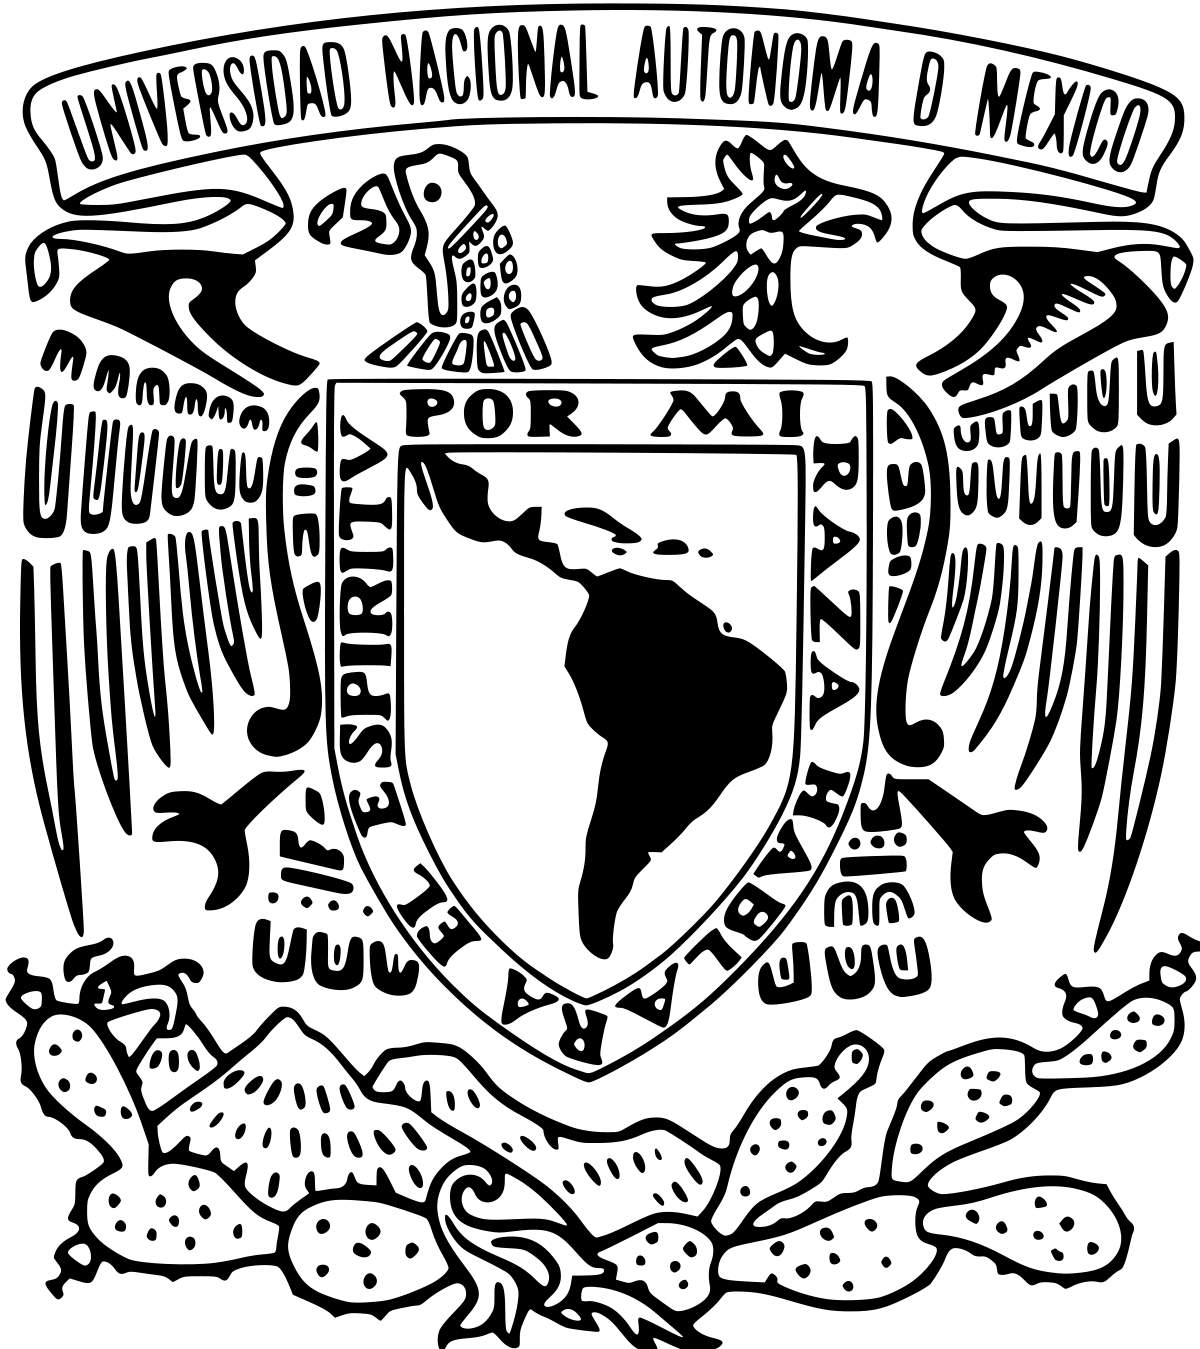
\includegraphics[height=3.4cm]{src/Img/Logo_UNAM.png}
    	\end{center}
    \end{minipage}\hfill
    \begin{minipage}{10cm}
    	\begin{center}
    	\textbf{\large Universidad Nacional Autónoma de México}\\[0.1cm]
        \textbf{Facultad de Ciencias}\\[0.1cm]
        \textbf{Análisis de Algoritmos  $|$ 7083}\\[0.1cm]
        Tarea 3 : $|$ Programacion Dinamica\\[0.1cm]
        Sosa Romo Juan Mario $|$ 320051926 \\[0.1cm]
        25/09/24
    	\end{center}
    \end{minipage}\hfill
    \begin{minipage}{3cm}
    	\begin{center}
    		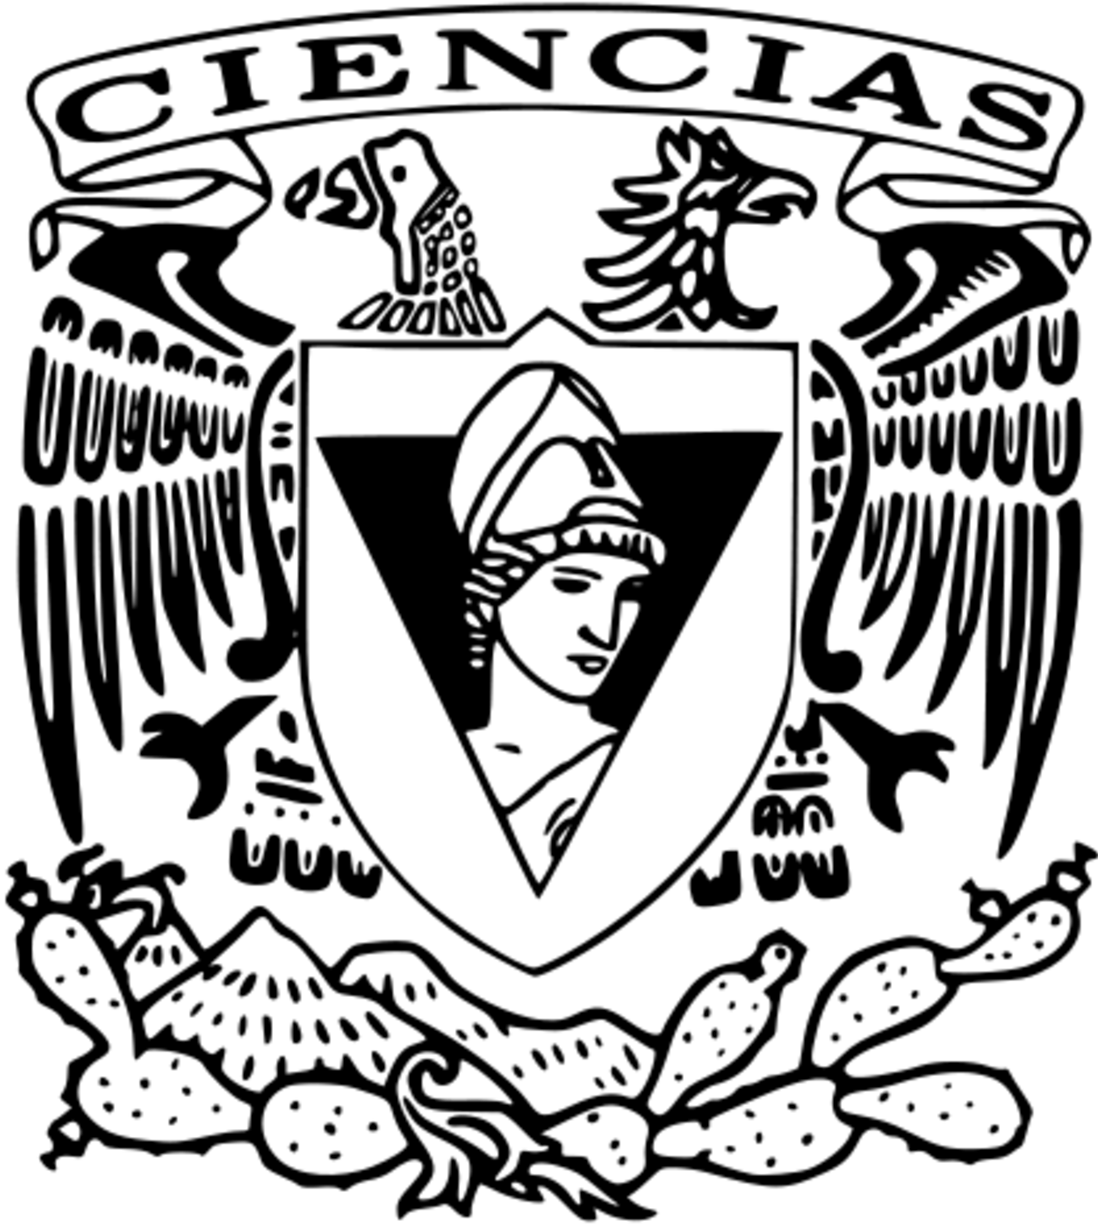
\includegraphics[height=3.4cm]{src/Img/Logo_FC.png}
    	\end{center}
    \end{minipage}
\end{center}


\rule{17cm}{0.1mm}


%------ Ejercicios -------- %
\begin{enumerate}
    \item \textbf{
    Un algoritmo glotón para regresar el cambio
    de n unidades usando el mínimo número de 
    monedas es el siguiente: Dar al cliente una
    moneda de mayor denominación, digamos d.
    Repite lo anterior para regresar el cambio 
    de n-d unidades.
}
\vspace{.3cm}

\textbf{
    Para cada una de las siguientes denominaciónes,
    determina si el algoritmo greedy antes mecionado
    mínimiza el número de monedas para dar el cambio.
    Si es así pruébalo, y si no lo es muestra un 
    contraejemplo.
}\vspace{.2cm}

\textcolor{red}{Esta probablemente no salio, si quiere no la califique pero la intente por si viene en el examen :v}
    \item \textbf{
    Construya el árbol de Huffman para codificar el siguiente texto:
    \begin{center}
        "El azote, hijo mío, se inventó para castigar afrontando al racional y para avivar la pereza del bruto que carece de razón; pero no para el niño decente y de vergüenza que sabe lo que le importa hacer y lo que nunca debe ejecutar, no amedrentado por el rigor del castigo, sino obligado por la persuasión de la doctrina y el convencimiento de su propio interés."
    \end{center}
}\vspace{.2cm}

No voy a explicar el algoritmo de Huffman, pues se vio en clase pero voy a hacer el procedimiento y luego mostrar con un árbol de Huffman online que esta bien hecho. \vspace{.2cm}

\textcolor{bibi}{Creamos el arbol de Huffman}
\begin{quote}
    \begin{itemize}
        \item \textbf{Paso 1:} Contamos la frecuencia de cada letra en el texto. (puede cambiar un poquito si consideras tabuladores o si yo conte mal xd)

        \begin{align*}
            \char`_ &: 65 \\
            e &: 39 \\
            a &: 34 \\
            o &: 27 \\
            r &: 25 \\
            n &: 21 \\
            i &: 17 \\
            l &: 15 \\
            t &: 13 \\
            d &: 13 \\
            c &: 12 \\
            p &: 11 \\
            s &: 9 \\
            u &: 9 \\
            v &: 5 \\
            g &: 5 \\
            z &: 4 \\
            , &: 4 \\
            m &: 4 \\
            y &: 4 \\
            b &: 4 \\
            q &: 4 \\
            \text{ó} &: 3 \\
            h &: 2 \\
            j &: 2 \\
            E &: 1 \\
            \text{í} &: 1 \\
            f &: 1 \\
            ; &: 1 \\
            \text{ñ} &: 1 \\
            \text{ü} &: 1 \\
            \text{é} &: 1 \\
            . &: 1 \\
        \end{align*}
        \item \textbf{Paso 2:} Creamos una lista con los nodos de cada letra y su frecuencia. (este paso literalmente solo es hacer eso entonces no muestro nada)
        \item \textbf{Paso 3:} Tomamos 2 arboles con las frecuencias mas bajas y los unimos en un nuevo arbol con la suma de las frecuencias, la raiz de este nuevo arbol es la suma de las frecuencias y los hijos son los arboles que unimos. Ademas, se etiqueta cada rama con un 0 si esta a la izquierda o un 1 si esta a la derecha, (este paso es el mas largo y tedioso, asi que solo muestro el resultado final)
        \item \textbf{Paso 4:} Repetimos el paso 3 hasta que solo quede un arbol. \vspace{.2cm}
    \end{itemize}

    No se si no se podia pero yo utilice un graficador en linea, igualmente el link del graficador es \href{https://www.csfieldguide.org.nz/en/interactives/huffman-tree/}{\underline{este}} y el resultado es este: \vspace{.2cm}

    \textbf{NOTA:} El graficador no le importa tanto si es izquierda o derecha al a hora de mostrar el resultado grafico (por eso aveces pone 0 a la derecha) pero internamente si lo esta haciendo solo lo dibuja al reves. \vspace{.2cm}
    \begin{center}
        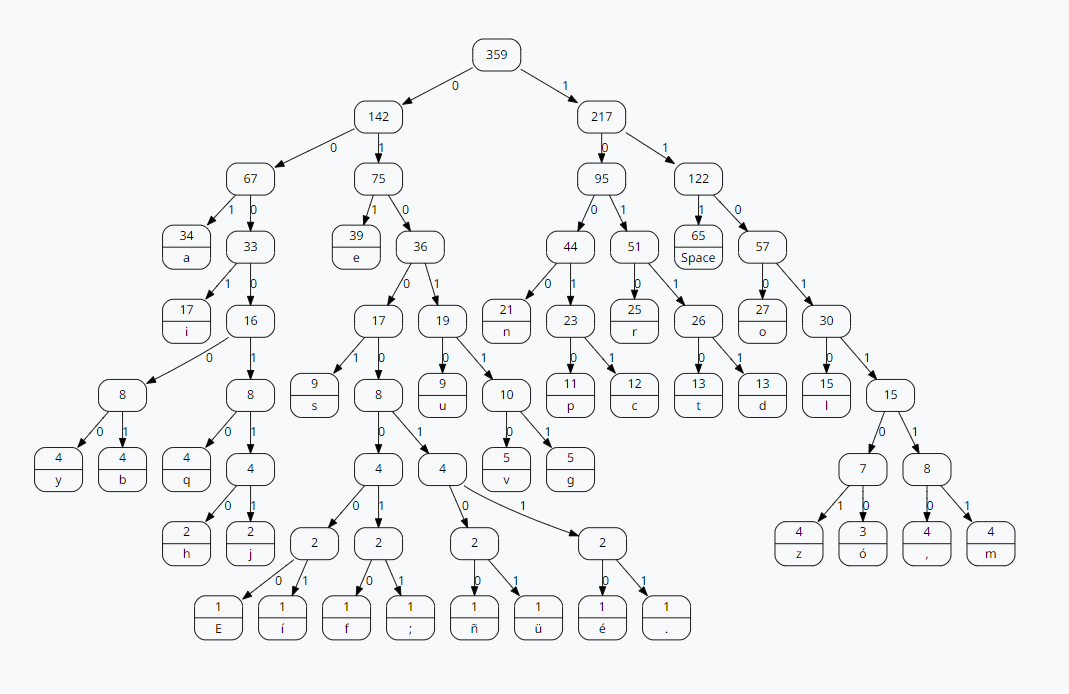
\includegraphics[width=14.9cm]{src/Img/ArbolHuffman.png}
    \end{center}

    Pero bueno por si acaso lo explico un poquito, hasta abajo vemos que los de frecuencia 1 se empezaron uniendo entre si generando arboles con raiz 2, a su vez se unieron entre si para generar arboles con raiz 4, aveces, cuando no hay arboles con la misma raiz, se toman los 2 de menor raiz digamos 8 y 9 se juntan para una raiz 17, y asi sucesivamente hasta que solo queda un arbol de raiz 359. \vspace{.2cm}

    Ahora, como mencionamos ir a la izquierda desde la raiz agrega un 0 a la codificacion del caracter y a la derecha un 1, entonces, si queremos saber la codificacion de una letra, simplemente seguimos el camino desde la raiz hasta la letra y anotamos los 0s y 1s que tomamos, este camino es unico aunque la codificacion no lo sea  (existen varias codificaciones de Huffman para este texto). Entonces por ejemplo el espacio tiene 111 como codificacion mientras que el . tiene una codificacion de 01000111 \vspace{.2cm} 
\end{quote}
    \item \textbf{Suponga que tenemos dos arreglos ordenados $A[1,\dots n]
\ y \ B[1, \dots, n]$ y un entero k. Describe un algoritmo para 
encontrar el \textit{k-ésimo} elemeneto en la unión de  \textit{A}
y \textit{B}. Por ejemplo, si $k=1$, tu algoritmo debe regresar el
elemento más pequeño de $A \cup B$; si $k=n$, tu algoritmo debe 
regresar la mediana de $A \cup B$. Puedes suponer que los arreglos 
no contienen duplicados. Tu algoritmo debe tener complejidad de tiempo
$\Theta (log \, n)$. Hint: Primero resuelve el caso especial k=n.}
    \item \textbf{Sea \textit{A} un arreglo de n númreos enteros distintos. Suponga
que \textit{A} tiene la siguiente propiedad: existe un indice $1 \leq k \leq
n$ tal que $A[1],\dots,A[k]$ es una secuencia incremental y $A[k+1],\dots,
A[n]$ es una secuencia decremental.}\\
    \item \textbf{Usted tiene que ordenar una serie $\Sigma_n$ de $n$ números, tales que todos son 0 ó 1. La única operación que puede hacer es comparar dos números cualesquiera $x$ y $y$, y cada que los compara recibe la respuesta $x < y$, $x = y$, or $x > y$.}\vspace{.2cm}
    \item \textbf{Se dice que un arreglo A[1,...,n] es k-ordenado si este puede ser dividido en k bloques cada uno de tamaño $\frac{n}{k}$ aproximadamente, tal que todos los elementos en cada bloque son mas grandes que el bloque anterior y mas pequeños que los elementos del bloque siguiente. Los elementos en cada bloque podrían no estar ordenados. Por ejemplo, el siguiente arreglo es 4-ordenado:
\begin{align*}
    1,2,4,3 \,|\, 7,6,5 \,|\, 10,11,9,12 \,|\, 15,13,16,14\\
\end{align*}}


    \item \textbf{Considera el siguiente algoritmo para ordenar:
\begin{center}
        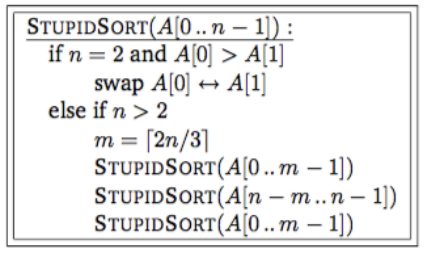
\includegraphics[width=5cm]{src/Img/stupidSort.png}\\
\end{center}}

    \item \textbf{Dado un arreglo $A$ con $n$ enteros positivos y negativos.}\vspace{.2cm}

\textcolor{bibi}{}
\begin{quote}
\end{quote}
    \begin{enumerate}
        \item \textbf{Suponiendo que puede cambiar de posición a las personas ¿Se puede resolver el problema con a lo mas una orden? Explique.}\\

Si, asumiendo que el mover de posición no cuenta como una orden, seria poner a todos los que tengan de una forma de un lado y los que lo tengan de la otra del lado contrario, así podríamos dar la orden de tomar uno de los 2 lados y pedirles a todos hasta el ultimo de esa forma que se cambien la gorra hacia el lado opuesto y tendríamos a todos de manera uniforme, (no se si entendí bien esta pregunta xd).\\
        \item \textbf{Dise\~na un algoritmo de programaci\'on din\'amica eficiente que determine si $Z$ es un \textit{shuffle} de $X$ y $Y$. \textit{Hint}: Los valores de la matriz de programaci\'on din\'amica que construyas, podr\'ian ser valores booleanos y no num\'ericos.}\vspace{.2cm}

El problema se parece bastante a la subcadena creciente mas grande.
La idea es usar una matriz de $|X|+1$ filas y $|Y|+1$ columnas, 
donde la celda $(i,j)$ indica si los primeros $i+j$ caracteres de $Z$
son un \textit{shuffle} de los primeros $j$ caracteres de $X$ y 
los primeros $i$ caracteres de $Y$. (podemos cambiar cual es quien pero asi lo hice) \vspace{.2cm}
    
\textcolor{bibi}{Usando matriz y programaci\'on din\'amica:}\vspace{.2cm}
\begin{quote}

    Podemos empezar verificando que $|X|+|Y|=|Z|$, si no es asi entonces
    no puede ser un \textit{shuffle} de $X$ y $Y$. \vspace{.2cm}

    Tenemos entonces que nuestra matriz se va a ver algo as\'i:

    \begin{table}[H]
        \centering
        \begin{tabular}{lllllll}
                &                              &                       & $x_0$                 & $x_1$                 & $\dots$               & $x_n$                 \\
                & i/j                          & 0                     & 1                     & 1                     & $\dots$               & n                     \\ \cline{3-7} 
                & \multicolumn{1}{l|}{0}       & \multicolumn{1}{l|}{1} & \multicolumn{1}{l|}{} & \multicolumn{1}{l|}{} & \multicolumn{1}{l|}{} & \multicolumn{1}{l|}{} \\ \cline{3-7} 
        $y_0$   & \multicolumn{1}{l|}{1}       & \multicolumn{1}{l|}{} & \multicolumn{1}{l|}{} & \multicolumn{1}{l|}{} & \multicolumn{1}{l|}{} & \multicolumn{1}{l|}{} \\ \cline{3-7} 
        $y_1$   & \multicolumn{1}{l|}{2}       & \multicolumn{1}{l|}{} & \multicolumn{1}{l|}{} & \multicolumn{1}{l|}{} & \multicolumn{1}{l|}{} & \multicolumn{1}{l|}{} \\ \cline{3-7} 
        $\dots$ & \multicolumn{1}{l|}{$\dots$} & \multicolumn{1}{l|}{} & \multicolumn{1}{l|}{} & \multicolumn{1}{l|}{} & \multicolumn{1}{l|}{} & \multicolumn{1}{l|}{} \\ \cline{3-7} 
        $y_m$   & \multicolumn{1}{l|}{m}       & \multicolumn{1}{l|}{} & \multicolumn{1}{l|}{} & \multicolumn{1}{l|}{} & \multicolumn{1}{l|}{} & \multicolumn{1}{l|}{} \\ \cline{3-7} 
        \end{tabular}
    \end{table}

    Ahora vamos a ver como llenarla, primero por la definición que hicimos, el indice
    (i,j) sera 1 pues los primeros 0+0 caracteres de Z siempre seran shuffle de los primeros
    0 caracteres de X y los primeros 0 caracteres de Y. \vspace{.2cm}

    Para la primera fila, hay que checar que los primeros $j$ caracteres de $X$ sean iguales
    a los primeros $j$ caracteres de $Z$, si es asi, entonces la celda $(0,j)$ sera 1, si no
    entonces sera 0; para checar esto podemos checar si el caracter j es igual en ambos y despues
    checar si a la izquierda ya tenemos un 1. ( esto es equivalente a: M[0][j]=M[0][j-1] AND X[j-1]==Z[j-1]
    tenemos que restar 1 porque las cadenas tienen indice en 0 pero tambien lo puedes entender con cantidad
    de caracteres) \vspace{.2cm}

    Para la primera columna, es lo mismo que la fila pero con $Y$ y $Z$, esto se puede entender como
    M[i][0]=M[i-1][0] AND Y[i-1]==Z[i-1]. \vspace{.2cm}

    Ahora para el caso de en medio hay que checar que los primeros $i+j$ caracteres de $Z$ sean shuffle
    de los primeros $j$ caracteres de $X$ y los primeros $i$ caracteres de $Y$, esto se puede entender
    como M[i][j]=M[i-1][j] AND Y[i-1]==Z[i+j-1] OR M[i][j-1] AND X[j-1]==Z[i+j-1]. \vspace{.2cm}

    De manera general nuestra funcion quedaria algo asi:
    \scriptsize
    \begin{align*}
        M[i][j]=\begin{cases}
            1 & \text{si } i=0 \text{ y } j=0 \\
            (M[i-1][j] \text{ AND } Y[i-1]==Z[i+j-1]) \text{ OR } (M[i][j-1] \text{ AND } X[j-1]==Z[i+j-1]) & \text{si } i>0 \text{ y } j>0 \\
        \end{cases}
    \end{align*}

    Al final sabremos si $Z$ es un \textit{shuffle} de $X$ y $Y$ si $M[|Y|][|X|]=1$, ademas el camino
    para ir de la celda $(|Y|,|X|)$ a la celda $(0,0)$ nos dira cuales son los caracteres que se usaron. \vspace{.2cm}

    Este algoritmo tiene complejidad $O(|X|*|Y|)$ y usa $O(|X|*|Y|)$ memoria, esto pues la matriz es de tamaño
    $(|X|+1)*(|Y|+1)$ y se llena en cada celda una vez tomando $O(1)$ tiempo (checar arriba y abajo, tomar un indice de 
    una cadena y compararlo con el indice en otra cadena que puede ser O(1)). \vspace{.2cm}

    Para entender mejor checar el ejemplo de arriba.
\end{quote}


\newpage
    \end{enumerate}
\end{enumerate}

\textbf{}\vspace{.2cm}

\textcolor{bibi}{}
\begin{quote}
\end{quote}

\end{document}